\documentclass[]{report}
\usepackage{amsmath,amsfonts,graphicx}

\def\species{\mathrm{sp}}
\def\phase{\mathrm{ph}}
\def\massfrac{\chi}
\def\flux{\mathbf{F}}
\def\darcyvel{\mathbf{v}}
\def\energydens{\mathcal{E}}
\def\d{\mathrm{d}}

\newcommand{\uo}{\mbox{UO\textsubscript{2}}\xspace}

\setcounter{secnumdepth}{3}
\DeclareMathOperator{\erfc}{erfc}

\begin{document}


\title{Flow from a source in a 1D radial model}
\author{CSIRO}
\maketitle

\tableofcontents

\chapter{Similarity solution}

Flow from a source in a radial 1D problem admits a similarity solution that is valid for a
broad range of problems, including multi-component, multi-phase flow. Properties such as fluid
pressure, saturation and component mass fraction can all be characterised by the similarity
variable $\zeta = r^2/t$, where $r$ is the radial distance from the source, and $t$ is time.

This similarity solution can be used to verify simple 1D radial models of increasing complexity.

\chapter{Two phase immiscible flow}

The simplest test case that features a similarity solution is injection of a gas phase into a fully liquid
saturated model at a constant rate. Figure \ref{fig:theis_similarity_fig} shows the comparison of
similarity solutions calculated with either fixed radial distance or fixed time. In this case, good agreement
is observed between the two results for both liquid pressure and gas saturation. This example is included
in the automatic test suite.

\begin{figure}[htb]
\centering
\includegraphics[width=\textwidth]{theis_similarity_fig.pdf}
\caption{Comparison of similarity solutions. (a) Liquid pressure; (b) Gas saturation}
\label{fig:theis_similarity_fig}
\end{figure}

\chapter{Two phase miscible flow}

The similarity solution is also recovered even when including mutual dissolution of the gas and aqueous
phases. In this example, CO$_2$ is injected into a fully saturated reservoir at a constant rate, with
the phase conditions calculated using the WaterNCG fluid state material that implements the persistent
primary variable (in this case, the total mass fraction of CO$_2$ summed over all phases) Initially, there
is insufficient CO$_2$ to form a gas phase, with all injected CO$_2$ dissolving into the resident water.

After approximately 3000 s, enought CO$_2$ has been injected to form a gas phase, and the problem
evolves from a single liquid phase to one including both gas and liquid phases. Figure
\ref{fig:theis_similarity_waterncg_fig} shows the comparison of similarity solutions calculated with
either fixed radial distance or fixed time. In this case, good agreement is observed between the two
results for both primary variables (gas pressure and total mass fraction of CO$_2$). The similarity
solution is also observed in Figure \ref{fig:theis_similarity_waterncg_fig2} for both the calculated
gas saturation and the mass fraction of CO$_2$ dissolved in the water.

This example is included in the automatic test suite.

\begin{figure}[htb]
\centering
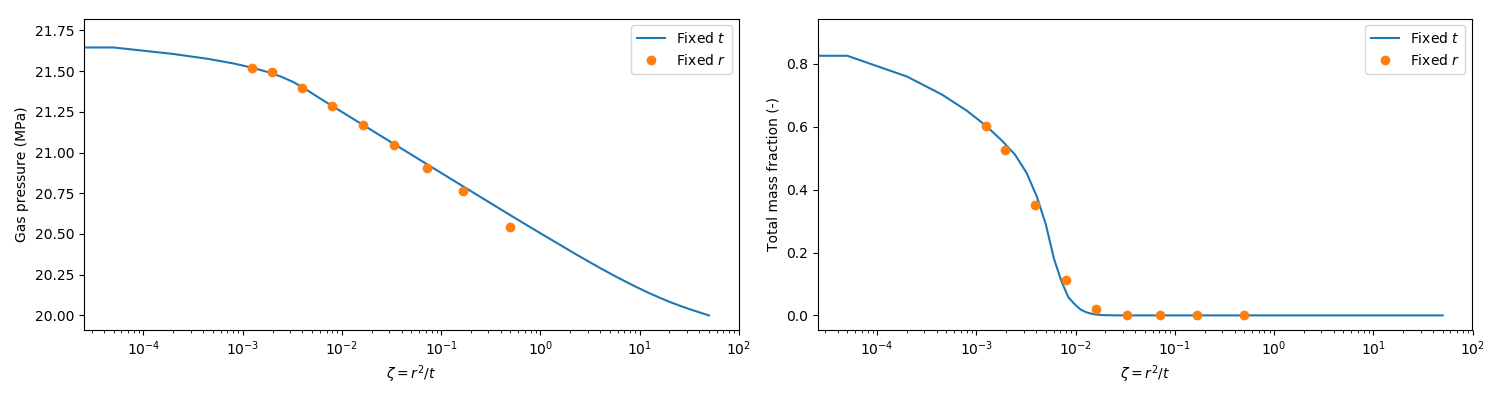
\includegraphics[width=\textwidth]{theis_similarity_waterncg_fig.pdf}
\caption{Comparison of similarity solutions for the water-NCG fluid state.
(a) Gas pressure; (b) Total mass fraction of CO$_2$.}
\label{fig:theis_similarity_waterncg_fig}
\end{figure}

\begin{figure}[htb]
\centering
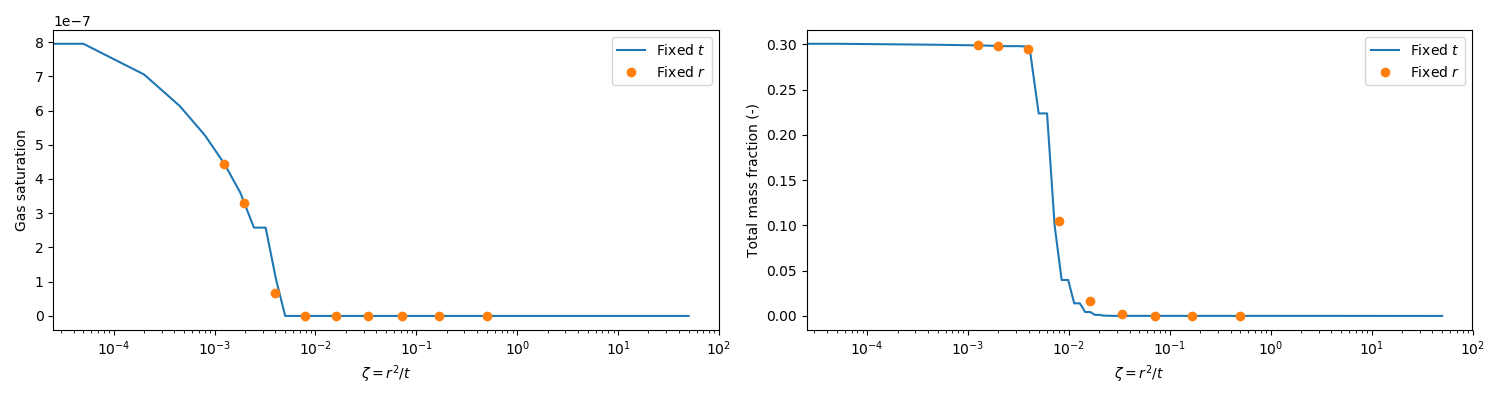
\includegraphics[width=\textwidth]{theis_similarity_waterncg_fig2.pdf}
\caption{Comparison of similarity solutions for the water-NCG fluid state.
(a) Gas saturation; (b) Dissolved CO$_2$ mass fraction.}
\label{fig:theis_similarity_waterncg_fig2}
\end{figure}

Similar results are obtained for CO$_2$ injection in brine, using the BrineCO2 fluid state material.
In this example, CO$_2$ is injected into a reservoir at a constant rate. Initially, the reservoir is
fully saturated with brine which has a salt mass fraction of 0.1. During the early injection period,
there is insufficient CO$_2$ to form a gas phase, with all injected CO$_2$ dissolving into the resident
brine.

After approximately 2000 s, enought CO$_2$ has been injected to form a gas
phase, and the problem evolves from a single liquid phase to one including both
gas and liquid phases. Note that this time is earlier than the problem with
water instead of brine, as the equilibrium saturation of CO$_2$ in  brine is
less than that in water. Figure \ref{fig:theis_similarity_brineco2_fig} shows
the comparison of similarity solutions calculated with either fixed radial
distance or fixed time. In this case, good agreement is observed between the two
results for both primary variables (gas pressure and total mass fraction of
CO$_2$). The similarity solution is also observed in Figure
\ref{fig:theis_similarity_brineco2_fig2} for both the calculated gas saturation
and the mass fraction of CO$_2$ dissolved in the water.

This example is included in the automatic test suite, but is marked heavy due to the
run time.

\begin{figure}[htb]
\centering
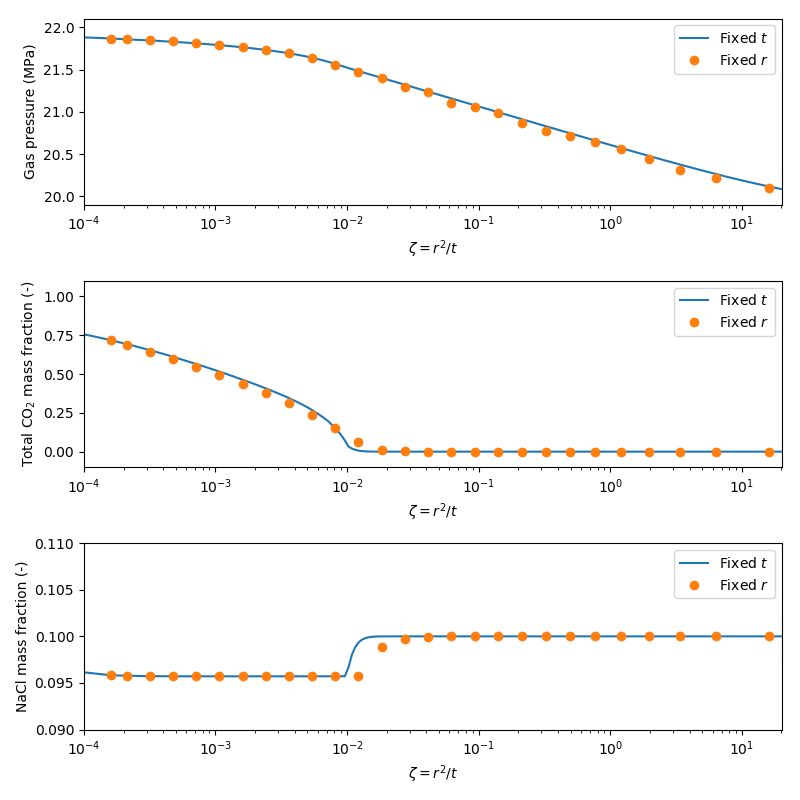
\includegraphics[width=\textwidth]{theis_similarity_brineco2_fig.pdf}
\caption{Comparison of similarity solutions for the brine-CO$_2$ fluid state.
(a) Gas pressure; (b) Total mass fraction of CO$_2$.}
\label{fig:theis_similarity_brineco2_fig}
\end{figure}

\begin{figure}[htb]
\centering
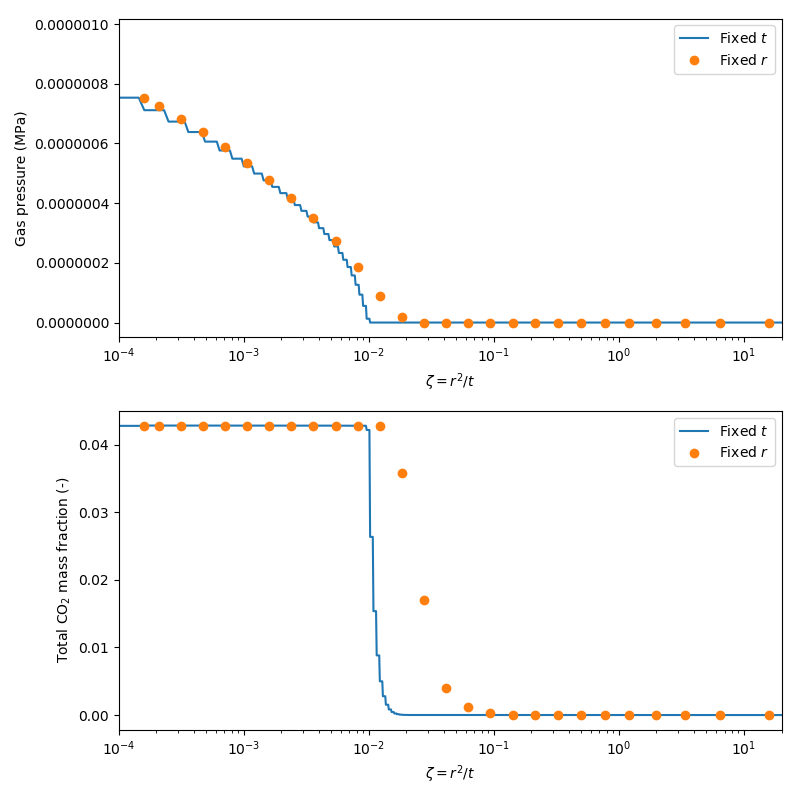
\includegraphics[width=\textwidth]{theis_similarity_brineco2_fig2.pdf}
\caption{Comparison of similarity solutions for the brine-CO$_2$ fluid state.
(a) Gas saturation; (b) Dissolved CO$_2$ mass fraction.}
\label{fig:theis_similarity_brineco2_fig2}
\end{figure}

\end{document}
